\documentclass{article}

\RequirePackage[svgnames]{xcolor}
\definecolor{UTorange}{RGB}{207, 83, 0} 
\definecolor{UTwhite}{RGB}{214, 210, 196}
\definecolor{UTgray}{RGB}{51, 63, 72}

\definecolor{UCLAblue}{RGB}{39, 116, 174} 
\definecolor{UCLAdark}{RGB}{0, 59, 92}
\definecolor{UCLAlight}{RGB}{218, 235, 254}
\definecolor{UCLAgold}{RGB}{255, 209, 0}

\definecolor{mered}{HTML}{882255}
\definecolor{megreen}{HTML}{004953}
\definecolor{mepink}{HTML}{AA4499}
\definecolor{rosequartz}{HTML}{F7CAC9}
\definecolor{serenity}{HTML}{92A8D1}

\definecolor{dark-red}{rgb}{0.4,0.15,0.15}
\definecolor{dark-blue}{rgb}{0.15,0.15,0.4}
\definecolor{medium-blue}{rgb}{0,0,0.5}

\usepackage{amsmath,amssymb, enumerate, tikz-cd,mathrsfs,hyperref,colortbl,bm}
\usepackage{graphicx, animate,lmodern}
\usepackage[export]{adjustbox}
\usepackage{cleveref}

\usepackage[outline]{contour}


%\usepgfplotslibrary{external}
 % \usetikzlibrary{external}
 % \tikzexternalize[prefix=tikz/]

\usepackage{float}
\usepackage{caption}
\usepackage{tikz}
\usepackage{tikz-3dplot}
\usepackage{pgfplots}
\pgfplotsset{compat=1.18}
\usetikzlibrary{scopes, angles, quotes, arrows.meta, calc, positioning, decorations.markings, decorations.pathreplacing,bending,shapes}
\usepgfplotslibrary{colormaps}

\newcommand\fixthis[1]{\textcolor{red}{#1}}

\newcommand{\R}{\mathbb{R}}
\newcommand{\C}{\mathbb{C}}
\newcommand{\Z}{\mathbb{Z}}
\newcommand{\Q}{\mathbb{Q}}
\newcommand{\F}{\mathbb{F}}
\newcommand{\N}{\mathbb{N}}

%my macros
\newcommand{\Sphere}{\mathbb{S}}
\newcommand{\TatekG}{\mathsf{Tate}(kG)}
\newcommand{\kGMod}{kG$-$\mathsf{Mod}}
\newcommand{\StMod}{\mathsf{StMod}}
\newcommand{\Mod}{\mathsf{Mod}}
\newcommand{\Top}{\textnormal{Top}}
\newcommand{\D}{\mathcal{D}}
\newcommand{\Ho}{\mathsf{Ho}}
\newcommand{\Hom}{\textnormal{Hom}}
\newcommand{\Ext}{\textnormal{Ext}}
\newcommand{\Tor}{\textnormal{Tor}}
\newcommand{\Cell}{\mathsf{Cell}}
\newcommand{\End}{\mathsf{End}}
\newcommand{\Spec}{\textnormal{Spec}}
\newcommand{\holim}{\textnormal{holim}}
\newcommand{\hocolim}{\textnormal{hocolim}}
\newcommand{\1}{\mathds{1}}
\newcommand{\Supp}{\textnormal{Supp}}
\newcommand{\supp}{\textnormal{supp}}
\newcommand{\Pic}{\textnormal{Pic}}
\newcommand{\pic}{\mathfrak{pic}}
\newcommand{\gl}{\mathfrak{gl}}
\newcommand{\Tot}{\textnormal{Tot}}
\newcommand{\CAlg}{\textnormal{CAlg}}
\newcommand{\Res}{\textnormal{Res}}
\newcommand{\CoInd}{\textnormal{CoInd}}


\tikzstyle{vector}=[-Latex,very thick, mered,line cap=round]
\tikzstyle{xline}=[UCLAblue,very thick]
\tikzstyle{yzp}=[canvas is zy plane at x=0]
\tikzstyle{xzp}=[canvas is xz plane at y=-1]
\tikzstyle{xyp}=[canvas is xy plane at z=1]
\def\tick#1#2{\draw[thick] (#1) ++ (#2:0.12) --++ (#2-180:0.24)}
\def\N{100}


\makeatletter %for the smooth/tension example
\tikzset{
	on each segment/.style={
		decorate,
		decoration={
			show path construction,
			moveto code={},
			lineto code={
				\path [#1]
				(\tikzinputsegmentfirst) -- (\tikzinputsegmentlast);
			},
			curveto code={
				\path [#1] (\tikzinputsegmentfirst)
				.. controls
				(\tikzinputsegmentsupporta) and (\tikzinputsegmentsupportb)
				..
				(\tikzinputsegmentlast);
			},
			closepath code={
				\path [#1]
				(\tikzinputsegmentfirst) -- (\tikzinputsegmentlast);
			},
		},
	},
}
\makeatother

\pgfplotsset{
	colormap={mesvtcolor}{
		rgb255=(145,168,209) 
		rgb255=(247,202,201)
	}%,
%	colormap/mesvtcolor,
}

\begin{document}
	
%	\begin{center}
%		\begin{tikzpicture}[scale=2, even odd rule]
%			\begin{axis}[view={65}{25},
%				axis lines=center,
%				%axis on top,
%				no marks,axis equal,
%				xmin=-3,xmax=3,ymin=-3,ymax=3,zmin=-1,zmax=2,
%				enlargelimits={upper=0.1},
%				xlabel={$x$},
%				ylabel={$y$},
%				zlabel={$z$}]
%				\addplot3[thick,
%				UCLAblue,samples=100,
%				domain=0.5:2,
%				y domain=0:0,
%				decoration={
%					markings,
%					mark=between positions 0.1 and 2 step 20mm with {\arrow{stealth}}
%				}, postaction=decorate
%				]
%				({cos(deg(2*pi*x))*e^x-1},{-sin(deg(pi*x))*e^x},{cos(deg(2*pi*x))});
%				
%				\addplot3[line width = 2.5pt,
%				white,samples=100,
%				domain=-.5:0.5,
%				y domain=0:0,
%				]
%				({cos(deg(2*pi*x))*e^x-1},{-sin(deg(pi*x))*e^x},{cos(deg(2*pi*x))});
%				
%				\addplot3[thick,
%				UCLAblue,samples=100,
%				domain=-.5:0.5,
%				y domain=0:0,
%				decoration={
%					markings,
%					mark=between positions 0.05 and 2 step 20mm with {\arrow{stealth}}
%				}, postaction=decorate
%				]
%				({cos(deg(2*pi*x))*e^x-1},{-sin(deg(pi*x))*e^x},{cos(deg(2*pi*x))});
%				
%				
%				% \def\NORM{sqrt((2*t)^2 + (4*t^3)^2)}
%				% \addplot3[thick, mered,-stealth,samples=8,variable=\t, domain=0:2,quiver={
%				%         u=-1*sin(deg(2*pi*t)), v=-1*cos(deg(2*pi*t)), w = 1,
%				%         scale arrows=0.2,
%				%     }]
%				%     ({cos(deg(2*pi*t))},{-1*sin(deg(2*pi*t))},{t});
%			\end{axis}
%		\end{tikzpicture}    
%	\end{center}
%	
%	\begin{center}
%		\begin{tikzpicture}[scale=2, even odd rule]
%			\begin{axis}[view={60}{30},
%				%axis on top,
%				no marks,axis equal,
%				xmin=-3,xmax=3,ymin=-3,ymax=3,zmin=-1,zmax=2,
%				enlargelimits={upper=0.1},
%				xlabel={$x$},
%				ylabel={$y$},
%				zlabel={$z$},zlabel style={rotate=-90}]
%				\coordinate (A) at (0,0,0);
%				\coordinate  (B) at (-5.48,4.48,-1);   
%				\addplot3[thick,
%				UCLAblue,samples=100,
%				domain=0.5:2,
%				y domain=0:0,
%				decoration={
%					markings,
%					mark=between positions 0.1 and 2 step 20mm with {\arrow{stealth}}
%				}, postaction=decorate
%				]
%				({cos(deg(2*pi*x))*e^x-1},{-sin(deg(pi*x))*e^x},{cos(deg(2*pi*x))});
%				
%				\addplot3[line width = 2.5pt,
%				white,samples=100,
%				domain=-.5:0.5,
%				y domain=0:0,
%				]
%				({cos(deg(2*pi*x))*e^x-1},{-sin(deg(pi*x))*e^x},{cos(deg(2*pi*x))});
%				
%				\addplot3[thick,
%				UCLAblue,samples=100,
%				domain=-.5:0.5,
%				y domain=0:0,
%				decoration={
%					markings,
%					mark=between positions 0.05 and 2 step 20mm with {\arrow{stealth}}
%				}, postaction=decorate
%				]
%				({cos(deg(2*pi*x))*e^x-1},{-sin(deg(pi*x))*e^x},{cos(deg(2*pi*x))});
%				\draw[thick, mered, -Latex] (A) --  node [above left] {$\bm{r}(1.5)$}(B);
%				\filldraw[black] (A) circle (2pt) node[below = .25cm]{$\bm{0}$};    
%				% \def\NORM{sqrt((2*t)^2 + (4*t^3)^2)}
%				% \addplot3[thick, mered,-stealth,samples=8,variable=\t, domain=0:2,quiver={
%				%         u=-1*sin(deg(2*pi*t)), v=-1*cos(deg(2*pi*t)), w = 1,
%				%         scale arrows=0.2,
%				%     }]
%				%     ({cos(deg(2*pi*t))},{-1*sin(deg(2*pi*t))},{t});
%			\end{axis}
%		\end{tikzpicture}    
%	\end{center}
%	
%	
%	\begin{center}
%		\begin{tikzpicture}[scale=2, even odd rule]
%			\begin{axis}[view={40}{20},
%				axis lines=center,
%				%axis on top,
%				no marks,axis equal,
%				xmin=-2,xmax=2,ymin=-2,ymax=2,zmin=-1,zmax=2,
%				enlargelimits={upper=0.1},
%				xlabel={$x$},
%				ylabel={$y$},
%				zlabel={$z$}]
%				\addplot3[thick,
%				UCLAblue,samples=100,
%				domain=-1:3,
%				y domain=0:0,
%				decoration={
%					markings,
%					mark=between positions 0.01 and 2 step 20mm with {\arrow{stealth}}
%				}, postaction=decorate
%				]
%				({-1*sin(deg(2*pi*x))},{cos(deg(2*pi*x))},{x});
%				
%				% \def\NORM{sqrt((2*t)^2 + (4*t^3)^2)}
%				% \addplot3[thick, mered,-stealth,samples=8,variable=\t, domain=0:2,quiver={
%				%         u=-1*sin(deg(2*pi*t)), v=-1*cos(deg(2*pi*t)), w = 1,
%				%         scale arrows=0.2,
%				%     }]
%				%     ({cos(deg(2*pi*t))},{-1*sin(deg(2*pi*t))},{t});
%			\end{axis}
%		\end{tikzpicture}    
%	\end{center}
%	
%	\begin{center}
%		\begin{tikzpicture}[scale=2, even odd rule]
%			\begin{axis}[view={40}{20},
%				axis lines=center,axis on top,
%				no marks,axis equal,
%				xmin=-2,xmax=2,ymin=-2,ymax=2,zmin=-1,zmax=2,
%				enlargelimits={upper=0.1},
%				xlabel={$x$},
%				ylabel={$y$},
%				zlabel={$z$}]
%				\addplot3[thick,
%				UCLAblue,samples=100,
%				domain=-1:3,
%				y domain=0:0,
%				decoration={
%					markings,
%					mark=between positions 0.01 and 2 step 4mm with {\arrow{stealth}}
%				}, postaction=decorate
%				]
%				({-1*sin(deg(2*pi*x))},{cos(deg(2*pi*x))},{x});
%				
%				% \def\NORM{sqrt((2*t)^2 + (4*t^3)^2)}
%				% \addplot3[thick, mered,-stealth,samples=8,variable=\t, domain=0:2,quiver={
%				%         u=-1*sin(deg(2*pi*t)), v=-1*cos(deg(2*pi*t)), w = 1,
%				%         scale arrows=0.2,
%				%     }]
%				%     ({cos(deg(2*pi*t))},{-1*sin(deg(2*pi*t))},{t});
%			\end{axis}
%		\end{tikzpicture}    
%	\end{center}
%	
%	\begin{center}
%		\begin{tikzpicture}[scale=2, even odd rule]
%			\begin{axis}[view={40}{20},
%				axis lines=center,
%				%axis on top,
%				no marks,axis equal,
%				xmin=-2,xmax=2,ymin=-2,ymax=2,zmin=-1,zmax=2,
%				enlargelimits={upper=0.1},
%				xlabel={$x$},
%				ylabel={$y$},
%				zlabel={$z$}]
%				\addplot3[thick,
%				UCLAblue,samples=100,
%				domain=-1:3,
%				y domain=0:0,
%				]
%				({-1*sin(deg(2*pi*x))},{cos(deg(2*pi*x))},{x});
%				
%				% \def\NORM{sqrt((2*t)^2 + (4*t^3)^2)}
%				% \addplot3[thick, mered,-stealth,samples=8,variable=\t, domain=0:2,quiver={
%				%         u=-1*sin(deg(2*pi*t)), v=-1*cos(deg(2*pi*t)), w = 1,
%				%         scale arrows=0.2,
%				%     }]
%				%     ({cos(deg(2*pi*t))},{-1*sin(deg(2*pi*t))},{t});
%			\end{axis}
%		\end{tikzpicture}    
%	\end{center}
%	
%	
%	
%	\begin{center}
%		\begin{tikzpicture}
%			\begin{axis}[
%				axis x line=middle,   
%				axis y line=middle,   
%				axis line style={<->},
%				xlabel={$x$},        
%				ylabel={$y$},      
%				xmin=-2,xmax=2,
%				ymin=-2.2,ymax=2.2,
%				grid=both,
%				axis equal,
%				]
%				\addplot [domain=0:1,samples=50,
%				UCLAblue, thick,
%				decoration={
%					markings,
%					mark=between positions 0.05 and 1 step 10mm with {\arrow{stealth}}
%				}, postaction=decorate]
%				({-1*sin(deg(2*pi*x))},{cos(deg(2*pi*x))}); 
%			\end{axis}
%		\end{tikzpicture}
%	\end{center}
%	
%	\begin{center}
%		\begin{tikzpicture}
%			\begin{axis}[
%				axis x line=middle,   
%				axis y line=middle,   
%				axis line style={<->},
%				xlabel={$x$},        
%				ylabel={$y$},      
%				xmin=-2,xmax=2,
%				ymin=-2.2,ymax=2.2,
%				grid=both,
%				axis equal,
%				]
%				\addplot [domain=0:1,samples=50,
%				UCLAblue, thick]
%				({-1*sin(deg(2*pi*x))},{cos(deg(2*pi*x))}); 
%			\end{axis}
%		\end{tikzpicture}
%	\end{center}
%	
%	\begin{center}
%		\begin{tikzpicture}
%			\begin{scope}[scale=2]
%				\node[label=below:$A$] (A) at (0,0) {};
%				\node[label=below:$B$] (B) at (2,0.25){};
%				\draw[UCLAblue] plot [smooth,tension=1]
%				coordinates {(A) (1,0) (1.14,-0.6) (0.5,-0.5) (0.5,0.5) (1.5,0) (B)}
%				[postaction={on each segment={draw,-{stealth[mered,bend]}}}];
%			\end{scope}
%			\draw [fill=black] (A) circle (1pt);
%			\draw [fill=black] (B) circle (1pt);
%		\end{tikzpicture}
%	\end{center}
%	
%	\def\xang{-13}
%	\def\zang{45}
%	\begin{tikzpicture}[x=(\xang:0.9), y=(90:0.9), z=(\zang:1.1)]
%		\message{^^JSynthesis 3D}
%		\def\xmax{8.8}         % max x axis
%		\def\ymin{-1.5}        % min y axis
%		\def\ymax{1.6}         % max y axis
%		\def\zmax{1.6}         % max z axis
%		\def\xf{1.17*\xmax}    % x position frequency axis
%		\def\A{(0.70*\ymax)}   % amplitude
%		\def\T{(0.335*\xmax)}  % period
%		\def\w{\zmax/11.2}     % spacing components
%		\def\ang{47}           % angle
%		\def\s{\ang/360*\T}    % time component
%		\def\x{\A*cos(\ang)}   % real component
%		\def\y{\A*sin(\ang)}   % imaginary component
%		
%		% COMPLEX PLANE
%		\begin{scope}[shift={(-1.6*\zmax,0,0)}]
%			\draw[black,fill=white,opacity=0.3,yzp]
%			(-1.25*\zmax,-1.25*\ymax) rectangle (1.4*\zmax,1.25*\ymax);
%			\draw[->,thick] (0,\ymin,0) -- (0,\ymax+0.02,0)
%			node[pos=1,left=0,yzp] {$z$};
%			\draw[->,thick] (0,0,-\zmax) -- (0,0,\zmax+0.02)
%			node[right=1,below=0,yzp] {$y$} coordinate (X);
%			%\node[scale=1,yzp] at (0,-\ymax,0) {Complex plane};
%			\draw[megreen, thick,yzp] (0,0) circle(0.991*\A) coordinate (O);
%			% \fill[mered,yzp] (\ang:{\A}) circle(0.07) coordinate({\s},{\y},{\x});
%			\node[megreen,above=1,yzp,scale=0.8] at ({\s},{\y},{\x}) {$\langle 0, \cos(t), \sin(t) \rangle$};
%			% \draw[vector,thick,yzp] (0,0) -- (\ang:{\A-0.03}) coordinate (R);
%			\tick{0,0,{\A}}{90};
%			\tick{0,0,{-\A}}{90};
%			\tick{0,{\A},0}{\zang};
%			\tick{0,{-\A},0}{\zang};
%		\end{scope}
%		
%		% IMAGINARY
%		\begin{scope}[shift={(0,0,1.9*\zmax)}]
%			\draw[black,fill=white,opacity=0.3,xyp]
%			(-1-0.5*\ymax,-1-1.2*\ymax) rectangle (1.10*\xmax,1.25*\ymax);
%			\draw[->,thick] (-0.3*\ymax,0,0) -- (\xmax,0,0)
%			node[below right=-2,xyp] {$x$};
%			\draw[->,thick] (0,\ymin,0) -- (0,\ymax,0)
%			node[left,xyp] {$z$};
%			\draw[UTorange, thick,samples=\N,smooth,variable=\t,domain=-0.05*\T:0.95*\xmax]
%			plot(\t,{\A*sin(360/\T*\t)},0);
%			%\node[below=0,xyp] at (0.4*\xmax,-\ymax,0) {Imaginary component};
%			% \fill[mered,xyp] ({\s},{\y}) circle(0.07) coordinate(I);
%			% \draw[vector,thick,xyp] ({\s},0) --++ (0,{\y-0.03});
%			\tick{0,{\A},0}{180};
%			\tick{0,{-\A},0}{180};
%			\tick{{\T},0,0}{90} node[right=-1,below,xyp] {\contour{white}{$\pi$}};
%			\tick{{2*\T},0,0}{90} node[right=-1,below,xyp] {\contour{white}{$2\pi$}};
%			\node[UTorange,below=0,xyp] at (0.4*\xmax,1.15*\ymax,0) {$\langle t, 0, \sin(t) \rangle$};
%		\end{scope}
%		
%		% REAL
%		\begin{scope}[shift={(0,-1.8*\zmax,0)}]
%			\draw[black,fill=white,opacity=0.3,xzp]
%			(-1-0.5*\ymax,-1.4*\ymax) rectangle (1.10*\xmax,1.25+1.25*\ymax);
%			\draw[->,thick] (-0.3*\ymax,0,0) -- (\xmax,0,0)
%			node[below right=-1,xzp] {$x$};
%			\draw[->,thick] (0,0,-\zmax) -- (0,0,\zmax)
%			node[left=-1,xzp] {$y$};
%			\draw[mered, thick,samples=\N,smooth,variable=\t,domain=-0.05*\T:0.95*\xmax]
%			plot(\t,0,{\A*cos(360/\T*\t)});
%			%\node[below=0,xzp] at (0.4*\xmax,-\ymax,0) {Real component};
%			% \fill[mered,xzp] ({\s},{\x}) circle(0.07) coordinate(R);
%			% \draw[vector,thick,xzp] ({\s},0) --++ (0,{\x-0.03});
%			\tick{0,0,{\A}}{180};
%			\tick{0,0,{-\A}}{180};
%			\tick{{\T},0,0}{\zang} node[left, above=.8,xzp] {$\pi$};
%			\tick{{2*\T},0,0}{\zang} node[left, above=.8,xzp] {$2\pi$};
%			\node[mered,above=0,xzp] at (0.3*\xmax,-\ymax,0) {$\langle t, \cos(t), 0 \rangle$};
%		\end{scope}
%		
%		% COMPONENTS
%		% \draw[mered!80!black,dashed]
%		%   (P) -- ({\s},{\y},{\x})
%		%   (I) -- ({\s},{\y},{\x+0.05})
%		%   ({\s},{\y-0.06},{\x}) -- (R);
%		\draw[->,black,thick] (-0.1*\ymax,0,0) -- (\xmax,0,0) node[below] {$x$};
%		\draw[->,black,thick] (0,\ymin,0,0) -- (0,\ymax+0.02,0) node[above] {$z$};
%		\draw[->,black,thick] (0,0,-\zmax) -- (0,0,\zmax+0.02) node[above] {$y$};
%		\foreach \i [evaluate={\tmin=max(-0.05*\T,(\i-0.05)*\T); \tmax=min(0.95*\xmax,(\i+1)*\T);}] in {0,...,2}{
%			%\draw[white,line width=1.2] (\tmin,0,0) -- (\tmax,0,0);
%			\draw[thick] (\tmin,0,0) -- (\tmax,0,0);
%			\draw[xline,samples=0.4*\N,smooth,variable=\t]
%			plot[domain=\tmin:\tmax](\t,{\A*sin(360/\T*\t)},{\A*cos(360/\T*\t)});
%		}
%		\draw[thick] (0,0,{0.9*\A}) -- (0,0,{\A});
%		% \fill[mered] ({\s},{\y},{\x}) circle(0.07) coordinate(Z);
%		% \draw[vector,thick] ({\s},0,0) --++ (0,{\y-0.03},{\x-0.03});
%		\draw[xline,samples=0.3*\N,smooth,variable=\t,domain=\s+0.03:\s+0.4*\T,line cap=round]
%		plot(\t,{\A*sin(360/\T*\t)},{\A*cos(360/\T*\t)});
%		\tick{{\T},0,0}{90};
%		\tick{{2*\T},0,0}{90};
%		\tick{0,0,{\A}}{90};
%		\tick{0,0,{-\A}}{90};
%		\tick{0,{\A},0}{\zang};
%		\tick{0,{-\A},0}{\zang};
%		\draw[mered!80!black,dashed]
%		({\s},{\y-0.06},{\x}) --++ (0,-0.2*\ymax,0);
%		
%	\end{tikzpicture}
%	
%	\begin{center}
%		\begin{tikzpicture}[scale=2]
%			
%			\begin{axis}[view={40}{20},
%				axis lines=center,
%				axis on top,
%				no marks,axis equal,
%				xmin=-2,xmax=2,ymin=-2,ymax=2,zmin=-1,zmax=2,
%				enlargelimits={upper=0.1},
%				xlabel={$x$},
%				ylabel={$y$},
%				zlabel={$z$}]
%				\addplot3[%opacity = 0.7, 
%				surf, colormap name=mesvtcolor, samples = 25, variable = \u, variable y = \v, domain = 0:360, y domain = -1:2]
%				({cos(u)}, {sin(u)}, {v});
%				
%			\end{axis}
%			
%		\end{tikzpicture}
%	\end{center}
	
%	\begin{tikzpicture}
%		\begin{axis}[
%			view={60}{30},
%			xlabel={$x$},
%			ylabel={$y$}, 
%			zlabel={$z$},zlabel style={rotate=-90},
%			xtick distance=2,
%			ytick distance=2,
%			xmin=-3, xmax=3,
%			ymin=-3, ymax=3, 
%			zmin=0, zmax=6,
%			restrict z to domain=-2:5,
%			enlargelimits={upper=0.1}]
%			\addplot3[domain=-2:2,surf,colormap name=mesvtcolor,samples=50] {x*x+y*y};
%		\end{axis}
%	\end{tikzpicture}  
	
	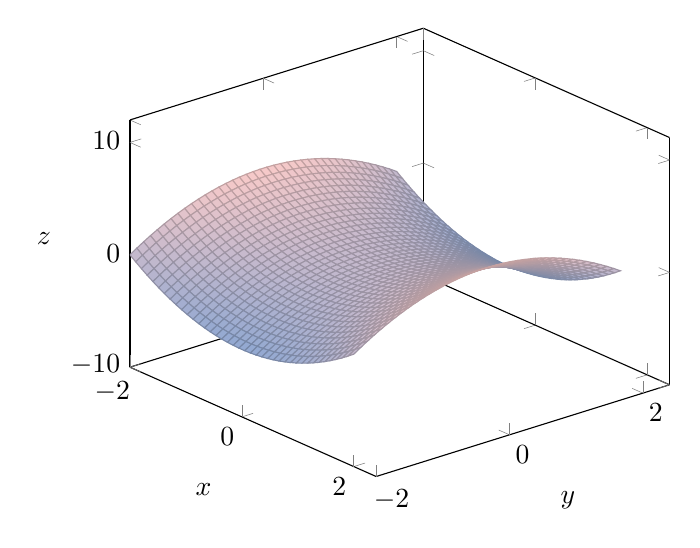
\begin{tikzpicture}
		\begin{axis}[
			view={50}{30},
			xlabel={$x$},
			ylabel={$y$},
			zlabel={$z$},zlabel style={rotate=-90},
			xtick distance=2,
			ytick distance=2,
			xmin=-2, xmax=2,
			ymin=-2, ymax=2, 
			zmin=-10, zmax=10,
			% restrict z to domain=-3:3,
			enlargelimits={upper=0.1}]
			\addplot3[domain=-2:2,surf,colormap name=mesvtcolor,samples=40] {x*x-y*y};
		\end{axis}
	\end{tikzpicture}  

 
	\begin{tikzpicture}[tdplot_main_coords, scale = 2]
		\begin{axis}[
			view={50}{30},
			xlabel={$x$},
			ylabel={$y$},
			zlabel={$z$},zlabel style={rotate=-90},
			xtick distance=2,
			ytick distance=2,
			xmin=0, xmax=10,
			ymin=0, ymax=10, 
			zmin=0, zmax=10,
			% restrict z to domain=-3:3,
			enlargelimits={upper=0.1}]
   \coordinate (P) at (5,5,8);
			\shade[ball color = lightgray,
    opacity = 0.5
] (P) circle (1cm);
\draw[dashed, black] (P) -- node[below, black]{$\varepsilon$} (4,2.8,8);
\draw[mered,fill = mered] (P) circle (0.5pt) node[below,mered]{$\bm{L}$};
\draw[megreen,fill = megreen] (4,6,9) circle (0.5pt) node[above,megreen]{$\bm{a_{M+1}}$};
\draw[megreen,fill = megreen] (4,5.5,8.5) circle (0.5pt);
\draw[megreen,fill = megreen] (4.5,5,8) circle (0.5pt);
\draw[fill = black] (4,10,9) circle (0.5pt) node[above]{$\bm{a_{1}}$};
\draw[fill = black] (1,3,4) circle (0.5pt) node[above]{$\bm{a_{M}}$};
\draw[fill = black] (10,3,4) circle (0.5pt) node[above]{$\bm{a_{2}}$};
\draw[fill = black] (5,3,4) circle (0.5pt);
\draw[fill = black] (7,6,4) circle (0.5pt);
\draw[fill = black] (1,3,9) circle (0.5pt);
		\end{axis}
	\end{tikzpicture}  
	
\end{document}